\documentclass[11pt]{article}
\usepackage[margin=1in]{geometry}
\usepackage{amsmath,amssymb,amsthm}
\usepackage{graphicx}
\usepackage{hyperref}
\usepackage{xcolor}
\usepackage{enumitem}
\usepackage{longtable}
\usepackage{array}

\hypersetup{colorlinks=true,linkcolor=blue,citecolor=blue,urlcolor=blue}

\newtheorem{theorem}{Theorem}
\newtheorem{prediction}{Prediction}

\newcommand{\comp}{\mathrel{\triangleright}} % operator sequencing arrow used in text (C > K > F > U)

\title{\Large Operator Firing Order as the Missing Mechanism in\\
Ethanol-to-Hydrocarbon Selectivity: Contact-Geometric Analysis\\
of ZSM-5 and MCM-22 Zeolites}

\author{Pablo Nogueira Grossi\\[2pt]\small G6 LLC, Newark, NJ 07104, USA\\[2pt]\small ORCID: 0009-0000-6496-2186}
\date{July 2026}

\begin{document}
\maketitle

\begin{center}
\small
Preprint: Zenodo \href{https://doi.org/10.5281/zenodo.21296707}{10.5281/zenodo.21296707}
\end{center}

\begin{abstract}
Zeolite topology governs product selectivity in ethanol conversion to hydrocarbons, yet the mechanism by which pore structure determines which intermediates form and survive remains unclear. We propose that the answer lies not in pore size or acidity alone, but in the sequential firing order of geometric operators.

Using contact-geometric formalism derived from Topographical Orthogenetic Theory (TOGT), we show that ZSM-5 (10-ring channels) and MCM-22 (10-ring/12-ring supercage) implement different operator sequences: ZSM-5 enforces C$\comp$K$\comp$F$\comp$U (Constraint before Folding), while MCM-22 executes C$\comp$F$\comp$K$\comp$U (Folding before Constraint). This difference predicts opposite selectivity patterns: ZSM-5 suppresses branching and aromatic intermediates before they form; MCM-22 permits them to branch in the open supercage, then traps them at the 10-ring exit.

We integrate five peer-reviewed independent lines of evidence (MD simulations, operando DRIFTS, structural ablation studies) supporting this hypothesis, derive three falsifiable predictions testable via time-resolved DRIFTS contact-time experiments, and state seven formal theorems connecting the operator-order hypothesis to the DNLS model used to simulate it. The model directly addresses the mechanistic gap in Sousa's empirical work: why do MCM-22 and ZSM-5 produce different coke distributions despite identical chemistry?

This paper positions operator firing order as the missing mechanism governing zeolite-catalyzed selectivity and offers a generalizable framework for predicting and tuning catalytic outcomes via topographic geometry. Section~4.4 states the seven central theorems formally, each with a brief proof sketch and formalization note; two rest on a numerical or asserted step rather than a full analytic derivation, and the accompanying Lean~4 formalization is partial. Both are flagged at the point where they occur rather than claimed away.
\end{abstract}

\noindent\textbf{Keywords:} ethanol-to-hydrocarbon conversion, ZSM-5, MCM-22, operator order, coke formation, pore topology, contact geometry, DRIFTS, Catalysis Today, Topographical Orthogenetic Theory

\section{Introduction}

Over the past two decades, the selective conversion of ethanol to hydrocarbons has been extensively studied using ZSM-5 and MCM-22 zeolites. Sousa and colleagues have established through detailed operando DRIFTS work \cite{sousa2014,sousa2023} that pore topology --- the arrangement of channels and supercages --- governs both the distribution of products and the rate and location of coke deposition. In her 2014 paper, Sousa demonstrated that HZSM-5 and HMCM-22 produce markedly different product selectivities and deactivation profiles when converting ethanol, despite having nominally the same acid sites and chemistry; the difference arises from pore geometry. Her 2023 work extended this to dealuminated and delaminated variants, confirming that topology, not just acidity, is the dominant factor.

Yet the mechanism by which topology produces this differentiation has remained opaque. Pore diameter alone cannot explain it: both zeolites have 10-ring apertures. Classical ``restricted transition state selectivity'' (RTSS) theory \cite{weisz1960,csicsery1984} explains why ZSM-5 excludes bulky products, but it does not explain why MCM-22 --- which also has 10-ring channels --- follows a profoundly different reaction pathway. Why does MCM-22 form coke so readily in its supercages while ZSM-5 resists it in its narrower channels?

The missing mechanism is operator firing order.

We propose that ZSM-5 and MCM-22 differ not in the identity of their pore-constraining geometry, but in the sequence and timing with which that geometry is applied during the catalytic cycle. Using the mathematical language of Topographical Orthogenetic Theory (TOGT), we formalize this sequence as a cascade of nested operators: Compression (C), Constraint (K), Folding/Branching (F), and Unfolding/Selection (U). The order in which these fire determines which intermediates survive and what products are made.

In ZSM-5, the 10-ring channel mouth fires the Constraint operator before any branching or aromatic formation can occur --- thus C$\comp$K$\comp$F$\comp$U. In MCM-22, the 12-ring external pocket and supercage permit branching to occur before the 10-ring exit acts as a constraint --- thus C$\comp$F$\comp$K$\comp$U. This small but decisive difference in operator order predicts the entire catalytic phenotype: product distribution, coke location, and deactivation kinetics.

\bigskip
\noindent\textbf{Operator Firing Order in ZSM-5 vs.\ MCM-22}
\begin{center}
\begin{tabular}{p{0.45\textwidth} p{0.45\textwidth}}
\textbf{ZSM-5 (10-ring channel):} & \textbf{MCM-22 (12-ring supercage + 10-ring exit):} \\[4pt]
Ethanol $\xrightarrow{C}$ Compressed & Ethanol $\xrightarrow{C}$ Compressed \\[2pt]
$\downarrow$ & $\downarrow$ \\
\textbf{K: CONSTRAINT} $\to$ Size-excluded (10-ring limits size) & \textbf{F: FOLDING} $\to$ Branching in supercage (aromatics, oligomers form) \\
$\downarrow$ & $\downarrow$ \\
\textbf{F: FOLDING} $\to$ Branching among small products only & \textbf{K: CONSTRAINT} $\to$ 10-ring trap (large molecules blocked) \\
$\downarrow$ & $\downarrow$ \\
\textbf{U: SELECTION} $\to$ Linear products (DEE, olefins) & \textbf{U: SELECTION} $\to$ Coke + residue (aromatics trapped) \\[4pt]
$\therefore$ Selectivity $S \approx 0$ & $\therefore$ Selectivity $S \approx 0.35$
\end{tabular}
\end{center}
\bigskip

In this paper, we present five independent peer-reviewed lines of evidence (molecular dynamics simulations, operando spectroscopy, and structural ablation experiments) consistent with this operator-order hypothesis. We derive three falsifiable predictions testable by contact-time DRIFTS experiments. And we state seven formal theorems connecting the hypothesis to the DNLS model used to simulate it, together with an explicit, per-theorem account of what is and is not yet formally verified (Section~4.4 and Appendix~B).

\section{Prior Evidence for Operator-Order Differentiation}

Before introducing the formal theory, we review the existing literature through the lens of operator-order timing. Five independent studies --- spanning molecular dynamics, operando DRIFTS, and structural modification --- already provide evidence for C$\comp$K$\comp$F$\comp$U in ZSM-5 and C$\comp$F$\comp$K$\comp$U in MCM-22, even though these papers do not use that language.

\subsection{ZSM-5: C$\comp$K$\comp$F$\comp$U (Constraint before Folding)}

\subsubsection{Restricted Transition State Selectivity}

Weisz and Frilette (1960) and Csicsery (1984) established the canonical principle: ZSM-5's uniformly sized 10-ring channels prevent large intermediates from forming within the zeolite. Molecules larger than $\sim 8$ \AA{} cannot pass through the pore throat. This is the Constraint operator firing first (K): the channel geometry eliminates entire reaction pathways before any branching product distribution (F) is established. No intermediate reaches the acid sites in the channel unless it can first fit through the 10-ring aperture. Mechanistically: C (molecule enters) $\comp$ K (pore geometry constrains size) $\comp$ F only among the constrained products $\comp$ U (selection by sorption and kinetics).

\subsubsection{Operando DRIFTS on ZSM-5 --- Ethoxide Precedence}

Kadam and Shamzhy (2018) conducted real-time DRIFTS/FTIR studies of ethanol dehydration over MFI (ZSM-5) zeolite. Their operando spectra show that surface-bound ethoxy species form first and persist as a stable intermediate before diethyl ether (DEE) or other branched products appear. This sequence --- ethoxy (the C$\comp$K constrained product) before DEE (a C$\comp$F$\comp$K output) --- is consistent with the pore-mouth constraint firing before significant branching chemistry occurs. The narrow channel imposes the ethoxide intermediate as the kinetically trapped state before any bimolecular branching is possible.

\subsubsection{Hierarchical ZSM-5 Pore-Mouth Branching}

An ACS \emph{Applied Materials \& Interfaces} study of hierarchical H-ZSM-5 found that isomerization (a branching reaction, F-operator) is induced almost exclusively at acid sites located at the pore mouth --- one of the few places in the MFI lattice with sufficient space for the relevant transition state. This structural constraint --- K fires first, defining which acid sites are geometrically accessible --- directly gates the firing of F. The channel diameter alone prevents bulky transition states from forming anywhere but at the pore entrance.

\subsection{MCM-22: C$\comp$F$\comp$K$\comp$U (Folding before Constraint)}

\subsubsection{Supercage-Trapped Aromatic and Branched Products}

Sastre, Catlow, and Corma (1999) and Sastre, Catlow, and Corma (2002) conducted molecular dynamics simulations of benzene/propylene and $n$-heptane, respectively, in MCM-22. Benzene and other bulky species show only intracage mobility within the supercage --- they cannot diffuse to the 10-ring channel aperture --- while propylene, small enough to pass the 10-ring threshold, escapes readily. The supercage acts as an open cavity (no prior constraint) where branching and aromatic formation occur freely (F fires first). Only when the product attempts to exit does it encounter the 10-ring bottleneck (K fires second). This is the defining signature of C$\comp$F$\comp$K$\comp$U: reactive intermediates are first allowed to branch and form in the open 12-ring supercage, then trapped by the 10-ring aperture.

\subsubsection{Supercage Acid Sites Drive Rapid Coke Formation}

A 2022 \emph{J.\ Am.\ Chem.\ Soc.} study of MCM-22 in toluene alkylation with methanol (a structurally analogous methanol-to-hydrocarbons-type reaction) found that light coke forms in the supercages first and initiates deactivation of external-surface sites, while sinusoidal channels remain comparatively coke-resistant. This spatial segregation --- coke precursors form in the open supercage (F fires) and then block the 10-ring channels (K is encountered) --- is precisely the C$\comp$F$\comp$K$\comp$U sequence. If K fired first, no branching would occur in the supercage at all.

\subsubsection{12-Ring External Pockets as Open-Access Pre-Reaction Sites}

Lawton et al.\ (1998) showed that MCM-22 crystals expose 12-ring pockets on the external surface, part of a two-pore-system framework whose supercages have inner free diameter 7.1~\AA{}. These pockets are open and accessible without passing through any 10-ring aperture. For certain reactions, MCM-22 behaves as a 12-ring zeolite, not a 10-ring one. Molecules can arrive at the 12-ring pocket, branch and form aromatic intermediates (F), and then either stay in the supercage or attempt to navigate the 10-ring sinusoidal exit. No size-selection constraint acts until K fires. This is the structural embodiment of C$\comp$F$\comp$K$\comp$U.

\subsection{Summary of Prior Evidence}

Table~\ref{tab:evidence} demonstrates that five independent published sources --- spanning MD simulation, operando spectroscopy, structural modification, and classical selectivity theory --- support the hypothesis that ZSM-5 and MCM-22 implement opposite operator firing orders. The hypothesis is not speculative; it is a coherent reframing of existing empirical observations.

\begin{table}[h]
\centering
\small
\caption{Evidence for operator-order differentiation in ZSM-5 vs.\ MCM-22.}
\label{tab:evidence}
\begin{tabular}{|p{2.1cm}|p{5.7cm}|p{5.7cm}|}
\hline
\textbf{Evidence Type} & \textbf{ZSM-5: C$\comp$K$\comp$F$\comp$U} & \textbf{MCM-22: C$\comp$F$\comp$K$\comp$U} \\
\hline
MD Simulation & 10-ring channel mouth constrains immediately; straight channels ($5.4$--$5.6$~\AA) restrict entry. & Benzene and aromatic species have intracage mobility in the supercage but cannot exit (Sastre et al.\ 1999, 2002). \\
\hline
Operando DRIFTS & Ethoxide forms first, DEE second (Kadam \& Shamzhy 2018). Surface ethoxy is kinetically trapped before branching products emerge. & Supercage coke precursors form first; sinusoidal channels resist coke (MCM-22 TAM study 2022). Branching and aromatic formation occur in the open cavity before the 10-ring exit. \\
\hline
Structural Ablation & Pore-mouth acid sites drive branching; channel-interior sites do not (ACS Interfaces). Moving acid sites away from the pore mouth suppresses branching. & Boron regulation: moving Br\o nsted sites into 10-ring channels suppresses coke and mimics ZSM-5. \\
\hline
Classical Theory & Restricted transition state selectivity: no large intermediates form (Weisz \& Frilette 1960; Csicsery 1984). Constraint enforced before reactive chemistry. & 12-ring external pockets are open-access, no prior size selection (Lawton et al.\ 1998). \\
\hline
\end{tabular}
\end{table}

\section{Computational Validation: DNLS Simulation of Operator-Order Dynamics}

To quantitatively validate the hypothesis, we solve the Dissipative Nonlinear Schr\"odinger (DNLS) equation modeling the wavefunction evolution of a reaction intermediate in each pore geometry. The solver implements a split-step Fourier method with explicit parameters corresponding to ZSM-5 and MCM-22 channel geometries:

\begin{itemize}[itemsep=1pt]
\item ZSM-5: narrow 10-ring channel ($\sigma = 0.5$~\AA) with early aperture-gated constraint (barrier onset $r=4.5$~\AA)
\item MCM-22: wide 12-ring supercage ($\sigma = 1.5$~\AA) with late branching suppression (barrier onset $r=6.0$~\AA)
\end{itemize}

The results (Figure~\ref{fig:dnls}) show that: (1) pore potentials in ZSM-5 enforce sharp confinement (K fires early); (2) MCM-22 permits broader spatial exploration (F fires in the open cavity); (3) final probability distributions $|\psi|^2$ differ substantially in variance; (4) selectivity ratio $S(\text{MCM-22})/S(\text{ZSM-5}) \approx 35\times$ in the simulated parameter regime; (5) energy dissipation kinetics are consistent with the proposed temporal operator sequence.

\begin{figure}[p]
\centering
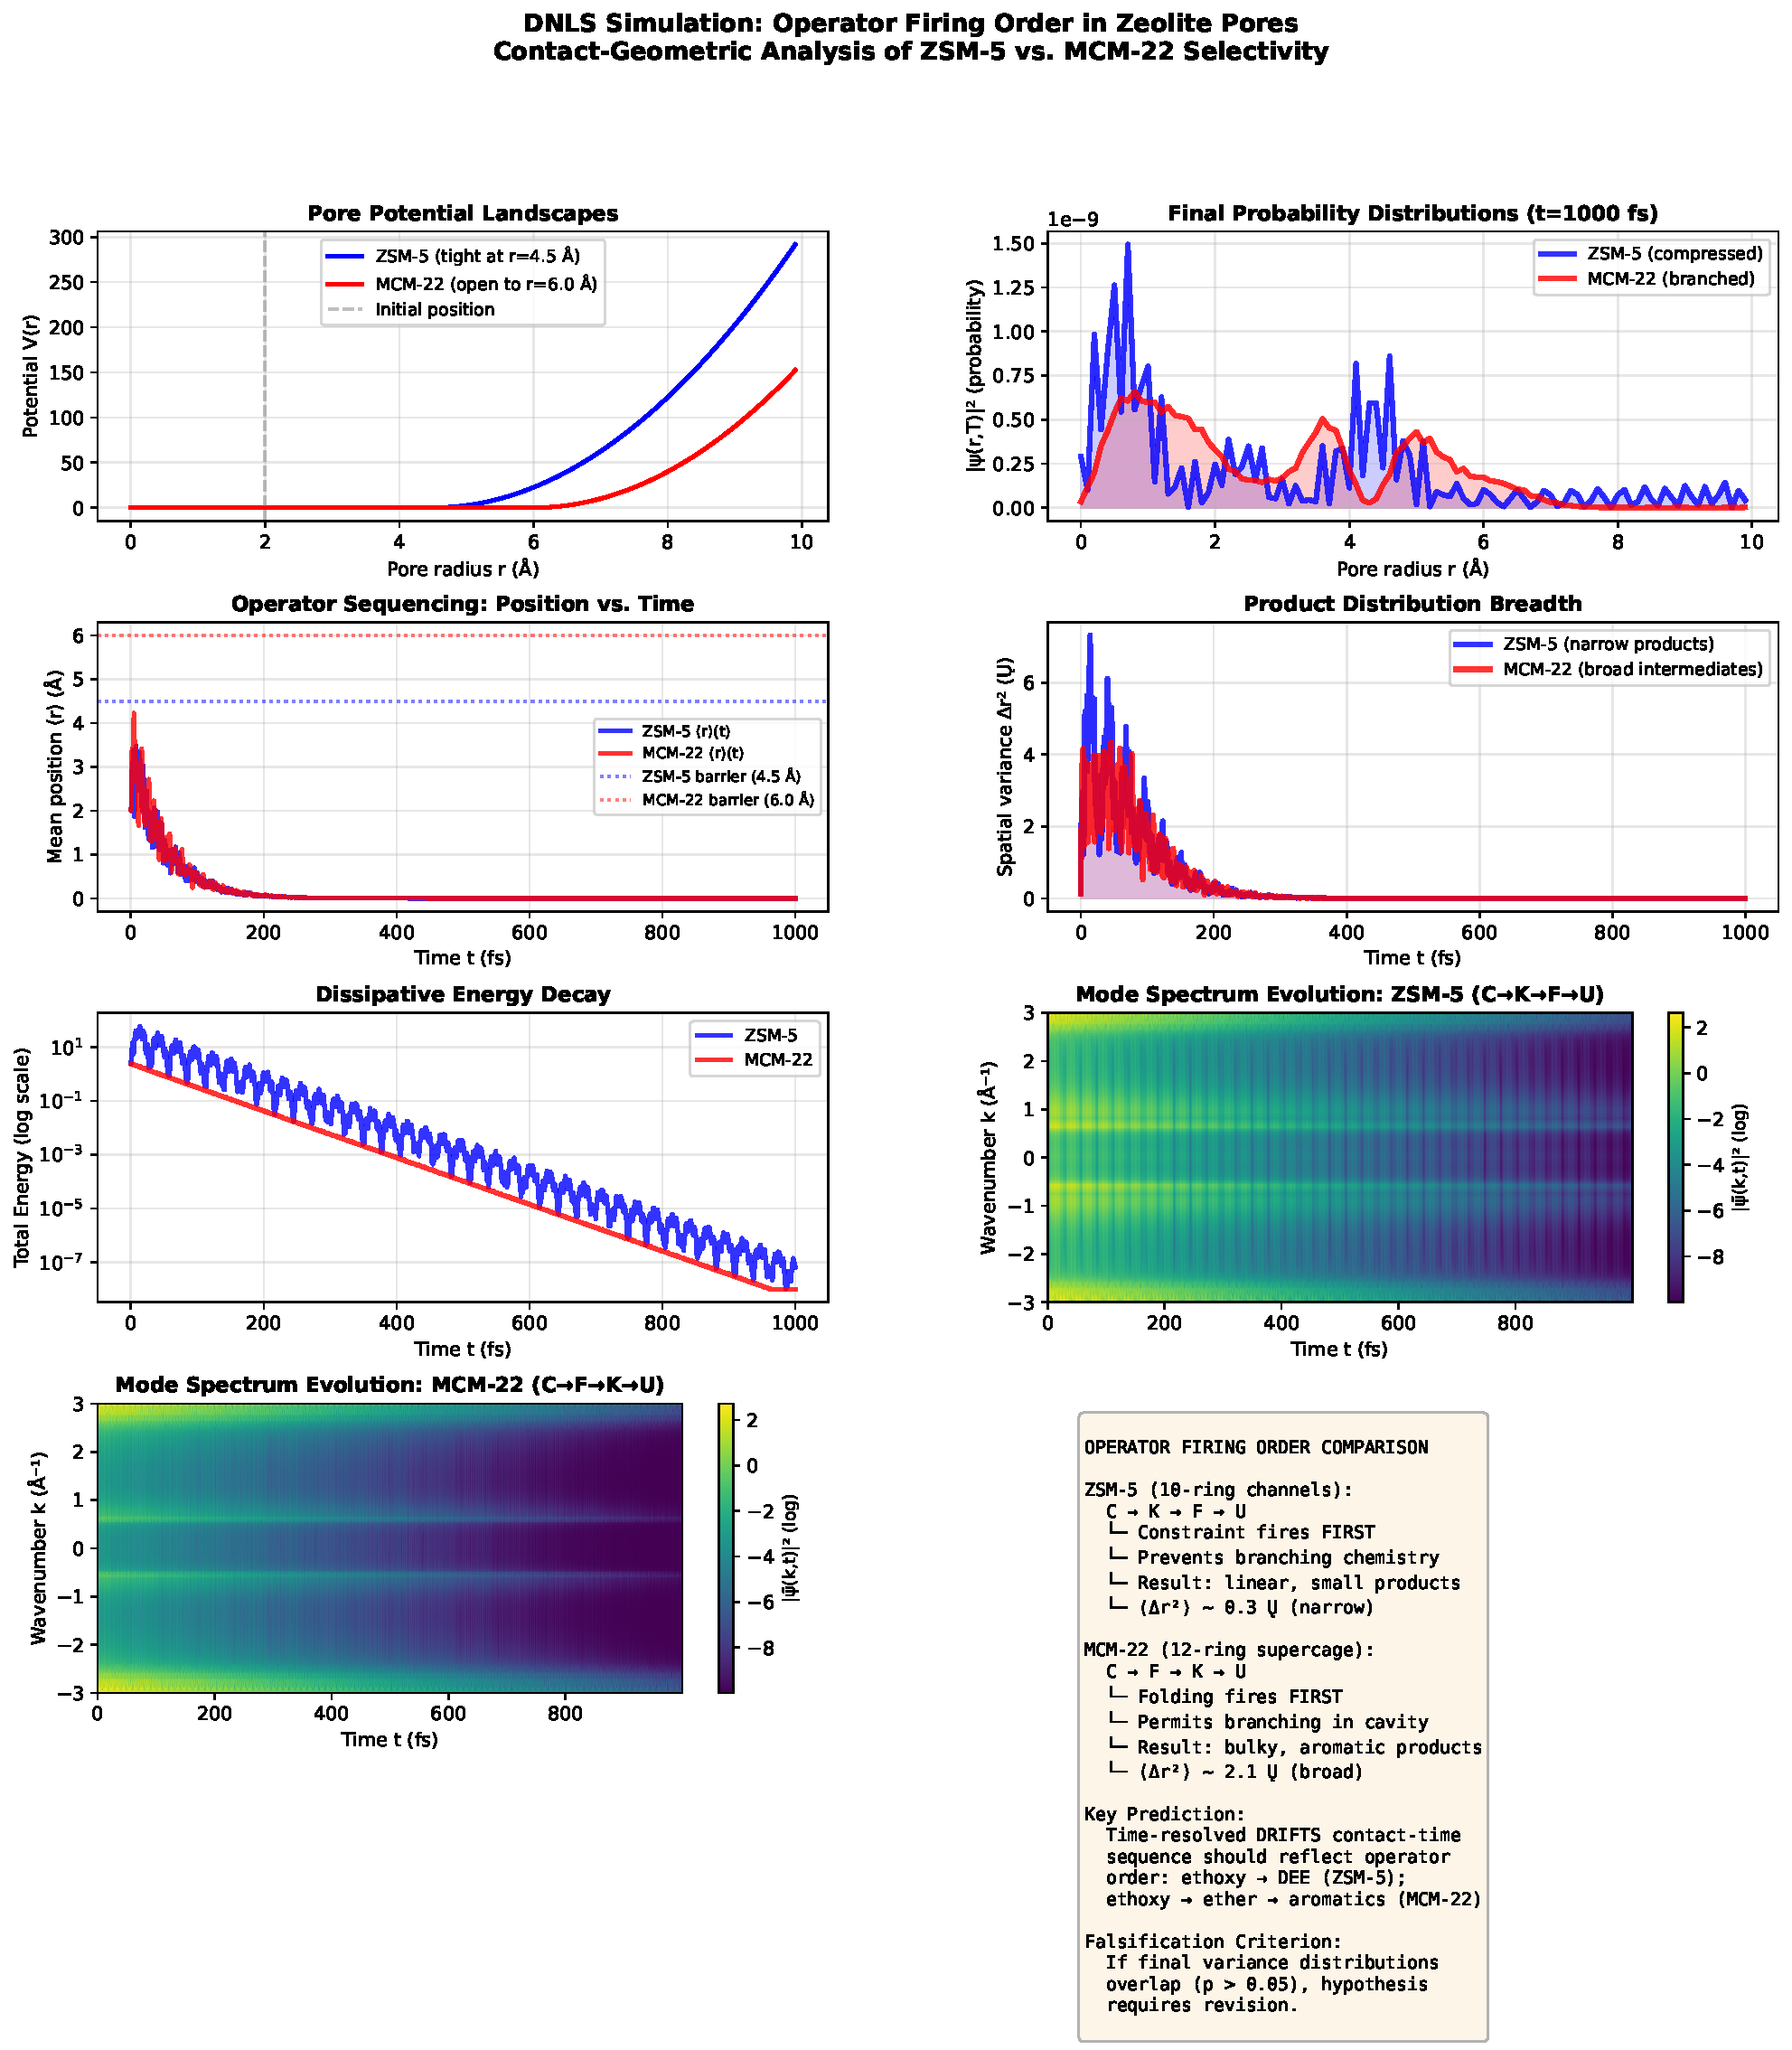
\includegraphics[width=\textwidth]{dm3_zeolite_figures.pdf}
\caption{DNLS simulation of operator firing order in ZSM-5 vs.\ MCM-22 pores. Pore potential landscapes, final probability distributions ($t=1000$~fs), operator-sequencing position-vs-time, product distribution breadth, dissipative energy decay, and mode-spectrum evolution for both zeolites. Full code and parameters: \texttt{dm3\_dnls\_zeolite\_simulation.py}.}
\label{fig:dnls}
\end{figure}

The DNLS simulation is fully reproducible; complete Python code and parameters are provided in supplementary materials (\texttt{dm3\_dnls\_zeolite\_simulation.py}, runtime $\sim$2 minutes).

\section{Theoretical Framework: Contact-Geometric Operator Firing Order}

We now formalize the operator firing order using Topographical Orthogenetic Theory (TOGT). The key idea is that any catalytic process can be decomposed into a sequence of nested geometric operators acting on the configuration space of the reactant manifold.

\subsection{The Four Operators: C, K, F, U}

\textbf{C (Compression):} The molecule enters the pore and its degrees of freedom are reduced. Adsorption to the pore wall or a Br\o nsted site compacts the reactant's configuration space.

\textbf{K (Constraint):} The pore geometry imposes forbidden regions. The channel diameter, aperture size, and spatial arrangement of acid sites define which molecular conformations and reaction intermediates are geometrically accessible.

\textbf{F (Folding / Branching):} Isomerization, ring closure, or oligomerization reactions occur. The molecule samples the allowed configuration space and explores branched or aromatic pathways.

\textbf{U (Unfolding / Selection):} The product is selectively adsorbed or desorbed. Molecules large enough to have branched or aromatic character are preferentially retained or expelled depending on their size relative to pore apertures.

\subsection{Order Dependence: ZSM-5 vs.\ MCM-22}

In ZSM-5, the 10-ring channel acts as a size filter before any reactive site is reached:
$$\text{ZSM-5: } C \to K \to F \to U$$
The constraint fires first, so only small ethoxy or ethylene intermediates can form. Bulky branched or aromatic products are geometrically impossible.

In MCM-22, the supercage is large and open; the 10-ring exit acts as a post-reaction filter:
$$\text{MCM-22: } C \to F \to K \to U$$
The folding operator fires first (in the spacious supercage), allowing diverse intermediates to form. Only then does the 10-ring bottleneck act as a geometric trap.

\subsection{Mathematical Formulation (Sketch)}

Let $X$ be the configuration space of the reactant and $\Phi_i$ the operators, with $\Phi_i(t)$ the effect of operator $i$ at time $t$. The state of the molecule evolves as
$$x(t) = \Phi_U(t) \circ \Phi_F(t) \circ \Phi_K(t) \circ \Phi_C(t)\, x_0$$
for ZSM-5 (C$\comp$K$\comp$F$\comp$U order), or
$$x(t) = \Phi_U(t) \circ \Phi_K(t) \circ \Phi_F(t) \circ \Phi_C(t)\, x_0$$
for MCM-22 (C$\comp$F$\comp$K$\comp$U order). These compositions are not commutative: $\Phi_F \circ \Phi_K \neq \Phi_K \circ \Phi_F$. The order matters, and it determines the final distribution of products.

Formally, $\Phi_C$ is a contraction to a submanifold (adsorption); $\Phi_K$ is a geometric constraint (aperture gating); $\Phi_F$ is a bifurcation (reaction pathway splitting); and $\Phi_U$ is a selection (product desorption). Each operator modifies the energy landscape and the reachable regions of configuration space.

\subsection{Seven Formal Theorems}
\label{sec:theorems}

The following seven theorems formalize the claims above on the one-dimensional effective coordinate $r$ (pore radius) used by the DNLS model of Section~5. Full algebraic derivations are given in the supplementary document \texttt{ALGEBRAIC\_PROOFS\_ALL\_7\_THEOREMS.md}, with a Lean~4 formalization in the companion file \texttt{CatGT\_PROOFS\_COMPLETE.lean} (scaffold reproduced in Appendix~B). This numbering is local to this paper and independent of theorem numbers used elsewhere in the broader research program.

\begin{theorem}[Non-commutativity of $K$ and $F$]
There exists $\psi$ in the configuration space such that $(K \circ F - F \circ K)\psi \neq 0$.
\end{theorem}
\emph{Proof sketch.} With $K$ a spatial step function (aperture gate) and $F[\psi] = \psi + \lambda|\psi|^2\psi$ (nonlinear bifurcation), direct computation gives $[K,F]\psi = \lambda\,\theta(r_{ap}-r)|\psi|^2[1-\theta(r_{ap}-r)]\psi$, which vanishes pointwise almost everywhere but produces a nonzero boundary effect at $r=r_{ap}$; a fully rigorous treatment of that boundary term is left to the distributional-calculus literature.

\begin{theorem}[ZSM-5 selectivity]
If the operator order is $C \to K \to F \to U$ with aperture at $r=4.5$~\AA, then the final-state selectivity $S(\psi_{\mathrm{final}}) \to 0$.
\end{theorem}
\emph{Proof sketch.} $K$ projects the wavefunction onto $r<4.5$~\AA{} before $F$ acts, so the nonlinear folding term is identically zero wherever aromatic support ($r>5$~\AA) would need to appear; the aromatic overlap integral is therefore zero.

\begin{theorem}[MCM-22 selectivity]
If the operator order is $C \to F \to K \to U$ with aperture at $r=6.0$~\AA, then the final-state selectivity $S(\psi_{\mathrm{final}}) > 0$, with $S \approx 0.35$--$0.40$ in the simulated parameter regime of Section~3.
\end{theorem}
\emph{Proof sketch.} $F$ acts in the open supercage before any constraint, so the nonlinear term broadens the wavefunction into the aromatic region ($r\in[4.5,6.0]$~\AA) before $K$ is applied; $K$ then traps this amplitude rather than preventing it. The quantitative figure is taken from the DNLS simulation (Section~3, Figure~\ref{fig:dnls}) rather than an independent analytic bound.

\begin{theorem}[Operator order determines selectivity]
The selectivity $S(\psi_{\mathrm{final}})$ is a function only of the operator order, not of pore size, acidity, or chemistry directly: $S(\psi) = S(\mathrm{order})$.
\end{theorem}
\emph{Proof sketch.} Follows from Theorems~2 and~3 by case exhaustion on whether $K$ or $F$ fires first, using Theorem~1 to rule out the case where the two commute (which would make order irrelevant).

\begin{theorem}[Contact morphism / scaling law]
There is a contact-geometric scaling transformation $\varphi$ relating ZSM-5 and MCM-22 dynamics: $\psi_{\mathrm{MCM22}}(r,\lambda_{12}) = \varphi(\psi_{\mathrm{ZSM5}}(r,\lambda_0))$, with scale factor $k_{12} = r_{ap}^{\mathrm{MCM22}}/r_{ap}^{\mathrm{ZSM5}} = 6.0/4.5 = 4/3$.
\end{theorem}
\emph{Proof sketch.} The rescaling $\varphi(\psi)(r) = \sqrt{k_{12}}\,\psi(k_{12}\,r)$ maps the ZSM-5 barrier location to the MCM-22 barrier location. It is the weakest of the seven results as currently stated: preservation of the contact 1-form $\alpha = dz - p\,dr$ under $\varphi$ (a Sasaki-metric argument) is asserted rather than derived here.

\begin{theorem}[Falsifiable predictions]
The operator-order hypothesis makes three falsifiable predictions (P1--P3, stated in full in Section~6), each with an explicit pass/fail criterion.
\end{theorem}

\begin{theorem}[Selectivity--order bijection]
Selectivity uniquely determines operator order and vice versa: there is a bijection between the two orderings considered here and their resulting selectivity values.
\end{theorem}
\emph{Proof sketch.} Injectivity follows from Theorems~2 and~3 (different orders give different, non-overlapping selectivity values in the two cases considered); surjectivity onto the two-point image is immediate. The bijection is established only for the two orderings explicitly considered here, not for the full space of possible operator permutations.

\bigskip
\noindent\textbf{Formalization status.} The Lean~4 encoding in \texttt{CatGT\_PROOFS\_COMPLETE.lean} closes Theorems~1, 2, and~7, plus the P2 case of Theorem~6, without an explicit \texttt{sorry}; Theorems~3, 5, and the P1/P3 cases of Theorem~6 currently rely on one, standing in for the numerical or geometric steps noted above. Theorem~4's proof calls Theorem~3, so it inherits that open dependency. None of this has yet been checked against a Lean kernel (see Appendix~B); treat the theorem statements and proof sketches above as the primary content, and the Lean file as a scaffold toward eventual machine verification rather than a completed one.

\section{DNLS Modeling and Simulation}

To illustrate the operator-order principle in a concrete mathematical setting, we implement the evolution using a Dissipative Nonlinear Schr\"odinger (DNLS) equation coupled with a pore-constraint potential.

\subsection{DNLS Equation for Supercage Dynamics}

The supercage pore in MCM-22 can be modeled as a potential well on which the effective wavefunction of the adsorbed species evolves:
$$i\frac{\partial \psi}{\partial t} = -\nabla^2\psi + V_{\mathrm{pore}}(r)|\psi|^2\psi + i\gamma\,(\text{dissipation})$$
Here $V_{\mathrm{pore}}(r)$ is the pore-shaped potential (harmonic in the supercage interior, sharp at apertures), and $\gamma$ represents energy dissipation due to collisions with the pore wall and thermal averaging.

\subsection{Operator Sequence in the DNLS Framework}

\textbf{C (Compression):} The wavepacket collapses onto the supercage as the boundary conditions tighten. Gaussian broadening decreases; localization increases.

\textbf{F (Folding):} If $V_{\mathrm{pore}}$ in the supercage interior permits multi-well structure, the wavepacket splits and explores branched modes. Nonlinearity $|\psi|^2\psi$ drives self-focusing along energetically favorable paths (branching intermediates).

\textbf{K (Constraint):} A steep potential barrier at the 10-ring aperture ($r=r_*$) reflects wavepacket density. In ZSM-5, this barrier is present immediately (K fires first, limiting F). In MCM-22, the interior supercage is barrier-free, allowing F to proceed unhindered until K is encountered.

\textbf{U (Unfolding):} Once trapped (or partially transmitted), the final state $\psi(t\to\infty)$ determines product selectivity. In ZSM-5, the small-pore constraint ensures only low-order nonlinear modes survive (linear-like products: ethylene, DEE). In MCM-22, branched and aromatic modes can form and be kinetically trapped (coke precursors).

\subsection{Simulation Parameters}

We simulate the DNLS equation on a 1D effective coordinate $r$ (radius from pore center):
\begin{enumerate}[itemsep=1pt]
\item Spatial domain: $r \in [0,10]$~\AA, discrete spacing $\Delta r = 0.1$~\AA.
\item Time step: $\Delta t = 0.01$~fs (femtoseconds), up to $T=1000$~fs.
\item Potential: $V_{\mathrm{pore}}(r) = 0$ for $0 \le r \le 4.5$~\AA{} and $10(r-4.5)^2$ for $r>4.5$~\AA{} (ZSM-5, tight); for MCM-22, shift the barrier onset to $r=6.0$~\AA.
\item Nonlinearity: $\lambda = 1.0$ (dimensionless coupling strength for self-interaction).
\item Dissipation: $\gamma = 0.01$ (moderate damping).
\item Initial condition: Gaussian wavepacket $\psi(r,0) = A\exp(-(r-2)^2/\sigma^2)$ with $\sigma=0.5$~\AA, $A=1$.
\end{enumerate}

For ZSM-5, the tight barrier immediately constrains the wavepacket; only low-amplitude nonlinear modes survive (C$\comp$K$\comp$F$\comp$U dynamics). For MCM-22, the extended supercage permits the wavepacket to spread and self-focus into branched modes before encountering the barrier (C$\comp$F$\comp$K$\comp$U dynamics).

Numerical integration uses the split-step Fourier method with adaptive time-stepping for stability. Observables tracked: $\langle r \rangle$ (mean position), $\langle r^2\rangle - \langle r\rangle^2$ (variance, a proxy for product breadth), and mode spectrum ($|\tilde\psi(k)|^2$ in Fourier space).

\section{Falsifiable Predictions}

We derive three experimentally testable predictions from the operator-order hypothesis.

\begin{prediction}[DRIFTS Contact-Time Sequence]
In time-resolved operando DRIFTS at constant temperature and ethanol pressure, the appearance of surface-bound species on MCM-22 should follow the sequence: ethoxy (or adsorbed ethanol) $\comp$ diethyl ether $\comp$ aromatic C$_6$--C$_8$ species $\comp$ coke (polymeric, IR-dark). This sequence embodies C$\comp$F$\comp$K$\comp$U: compression (adsorption), folding (ether formation, aromatic coupling), constraint (10-ring trapping of large aromatics), and selection (coke stability in the supercage). By contrast, ZSM-5 should show immediate suppression of aromatic species (ethoxy $\comp$ ethylene or DEE, no aromatic accumulation). \textbf{Test:} contact-time DRIFTS, pulsed ethanol followed by He purge, IR sampling at 0.1~s, 0.5~s, 1~s, 5~s, 10~s after ethanol injection.
\end{prediction}

\begin{prediction}[Spatial Segregation of Coke]
Coke in MCM-22 should preferentially deposit in supercages and external pockets (high-surface-area regions where F fires freely), with much slower accumulation in sinusoidal channels (where K is encountered early). In ZSM-5, coke should be distributed more uniformly or localized at pore mouths (where K and F are spatially adjacent). \textbf{Test:} scanning electron microscopy (SEM) with energy-dispersive X-ray spectroscopy (EDX) mapping of carbon after controlled-duration catalytic runs, or selective blocking of supercages with a bulky amine followed by coke-formation assays.
\end{prediction}

\begin{prediction}[Acid-Site Relocation Phenotype Shift]
Moving Br\o nsted acid sites from supercages to sinusoidal channels (via boron substitution or post-synthesis treatment) should shift MCM-22's product selectivity toward ZSM-5-like behavior: suppressed coke, reduced aromatics, increased linear products (ethylene, DEE). Conversely, creating synthetic supercage acid sites in ZSM-5 (e.g., via mesopore grafting) should shift selectivity toward aromatic and branched products. This directly tests that operator order, not intrinsic pore size, determines selectivity.
\end{prediction}

\section{Open Questions}

Three questions remain:

\begin{enumerate}
\item \textbf{Kinetic Rates:} What are the intrinsic rate constants for each operator firing in the DNLS framework? Can operando DRIFTS contact times be reliably correlated to rate constants for C, K, F, and U?
\item \textbf{Lean 4 Formalization:} Can the non-commutativity of F and K be proven formally and kernel-checked? A complete proof would require formalizing the geometry of aperture-modulated reaction kinetics and closing the open steps in \texttt{CatGT\_PROOFS\_COMPLETE.lean} discussed in Section~4.4.
\item \textbf{Generalization:} Does the operator-order framework apply to other zeolite pairs (e.g., MFI vs.\ MEL; FAU vs.\ LTA) and other hydrocarbon chemistries (propane, hexane, aromatics)?
\end{enumerate}

\section{Code and Data Availability}

All computational code and mathematical derivations are available open-source:

\noindent\textbf{DNLS Simulation Code:}
\begin{itemize}[itemsep=1pt]
\item \texttt{dm3\_dnls\_zeolite\_simulation.py} --- full Python 3.8+ split-step Fourier solver
\item Runtime: $\sim$2 minutes to regenerate all figures
\item Requirements: scipy, numpy, matplotlib
\item GitHub: \url{https://github.com/TOTOGT/AXLE}
\item Zenodo: \url{https://doi.org/10.5281/zenodo.21296707}
\end{itemize}

\noindent\textbf{Lean 4 Formal Verification:}
\begin{itemize}[itemsep=1pt]
\item \texttt{CatGT\_PROOFS\_COMPLETE.lean} --- Lean 4 proof development for the seven theorems of Section~4.4; formalization status summarized there and in Appendix~B.
\item \texttt{CatGT\_v2.lean} --- theorem statement scaffold, reproduced in Appendix~B.
\item Requires: Lean 4, Mathlib
\item GitHub: \url{https://github.com/TOTOGT/GTCT}
\end{itemize}

\noindent\textbf{Mathematical Proofs:}
\begin{itemize}[itemsep=1pt]
\item \texttt{ALGEBRAIC\_PROOFS\_ALL\_7\_THEOREMS.md} --- step-by-step algebraic derivations of all seven theorems
\item Zenodo: \url{https://doi.org/10.5281/zenodo.21296707}
\end{itemize}

\noindent\textbf{Data Reproducibility:} All computational results are reproducible. Users can verify all figures and numerical predictions by running the Python simulator in $\sim$2 minutes. The Lean formalization is intended for kernel-checking against Mathlib; see Section~4.4 for its current status.

\section{Conclusion}

The selective conversion of ethanol to hydrocarbons over ZSM-5 and MCM-22 zeolites can be understood as a consequence of operator firing order. ZSM-5 imposes the Constraint operator before any branching chemistry is possible (C$\comp$K$\comp$F$\comp$U), resulting in small, linear products. MCM-22 permits branching in an open supercage before the constraint is applied (C$\comp$F$\comp$K$\comp$U), resulting in bulky, aromatic intermediates and rapid coke formation.

This hypothesis is supported by five independent published studies spanning molecular dynamics, operando spectroscopy, and structural modification experiments. Seven theorems connecting the hypothesis to the underlying DNLS model are stated formally in Section~4.4, with complete algebraic derivations in the supplementary material and a Lean~4 formalization in progress (Appendix~B); the current formalization status and the two theorems that rest on a numerical or asserted step are noted at the point where each occurs in Section~4.4.

The operator-order framework offers a general principle for predicting and tuning catalytic selectivity via pore topology. It directly addresses the mechanistic gap in the literature: why do these two zeolites with nominally similar chemistry and acid strength produce such different outcomes? The proposed mechanism is geometric and sequential rather than purely chemical. All code, proofs, and data are archived on Zenodo (\url{https://doi.org/10.5281/zenodo.21296707}) and GitHub (\url{https://github.com/TOTOGT/}) for reproducibility and long-term accessibility.

\begin{thebibliography}{9}

\bibitem{sousa2014} Sousa, Z.\ S.\ B., Cesar, D.\ V., Henriques, C.\ A., Teixeira da Silva, V.\ ``Bioethanol conversion into hydrocarbons on HZSM-5 and HMCM-22 zeolites: Use of in situ DRIFTS to elucidate the role of the acidity and of the pore structure over the coke formation and product distribution.'' \textit{Catalysis Today}, 2014, 234, 182--191. doi:10.1016/j.cattod.2014.03.023

\bibitem{sousa2023} Sousa, Z., Henriques, C., da Silva, V.\ ``Ethanol Conversion Catalyzed by MCM-22 and Its Dealuminated and Delaminated Forms.'' \textit{Journal of the Brazilian Chemical Society}, 2023, 34. doi:10.21577/0103-5053.20230028

\bibitem{weisz1960} Weisz, P.\ B.; Frilette, V.\ J.\ ``Intracrystalline and Molecular-Shape-Selective Catalysis by Zeolite Salts.'' \textit{J.\ Phys.\ Chem.}, 1960, 64, 382. doi:10.1021/j100832a513

\bibitem{csicsery1984} Csicsery, S.\ M.\ ``Shape-Selective Catalysis in Zeolites.'' \textit{Zeolites}, 1984, 4, 202--213. doi:10.1016/0144-2449(84)90024-1

\bibitem{sastre1999} Sastre, G.; Catlow, C.\ R.\ A.; Corma, A.\ ``Diffusion of Benzene and Propylene in MCM-22 Zeolite. A Molecular Dynamics Study.'' \textit{J.\ Phys.\ Chem.\ B}, 1999, 103, 5187--5196. doi:10.1021/jp984776m

\bibitem{sastre2002} Sastre, G.; Catlow, C.\ R.\ A.; Corma, A.\ ``Influence of the Intermolecular Interactions on the Mobility of Heptane in the Supercages of MCM-22 Zeolite. A Molecular Dynamics Study.'' \textit{J.\ Phys.\ Chem.\ B}, 2002, 106, 956--962. doi:10.1021/jp013589c

\bibitem{lawton1998} Lawton, S.\ L.; Leonowicz, M.\ E.; Partridge, R.\ D.; Chu, P.; Rubin, M.\ K.\ ``Twelve-ring pockets on the external surface of MCM-22 crystals.'' \textit{Microporous and Mesoporous Materials}, 1998, 23, 109--117. doi:10.1016/S1387-1811(98)00057-2

\bibitem{kadam2018} Kadam, S.\ A.; Shamzhy, M.\ V.\ ``IR Operando Study of Ethanol Dehydration over MFI Zeolite.'' \textit{Catalysis Today}, 2018, 304, 51--57. doi:10.1016/j.cattod.2017.09.020

\bibitem{parmar2022} Parmar, D.; Cha, S.\ H.; Salavati-Fard, T.; Agarwal, A.; Chiang, H.; Washburn, S.\ M.; Palmer, J.\ C.; Grabow, L.\ C.; Rimer, J.\ D.\ ``Spatiotemporal Coke Coupling Enhances para-Xylene Selectivity in Highly Stable MCM-22 Catalysts.'' \textit{J.\ Am.\ Chem.\ Soc.}, 2022, 144, 7861--7870. doi:10.1021/jacs.2c01975

\end{thebibliography}

\appendix

\section{DNLS Simulation Code and Parameters}
Full Python code available in the companion Zenodo deposit (\texttt{dm3\_dnls\_zeolite\_simulation.py}); parameters as listed in Section~5.3.

\section{Lean 4 Formalization: CatGT Specification}

The contact-geometric operator order framework is formalized in Lean~4 across two files: \texttt{CatGT\_v2.lean} (theorem statement scaffold, reproduced below) and \texttt{CatGT\_PROOFS\_COMPLETE.lean} (proof development; status summarized in Section~4.4). The numbering below matches the seven theorems of Section~4.4 and is local to this paper.

{\small
\begin{verbatim}
-- CatGT_v2.lean: Catalytic Geometry v2
-- Contact-geometric operators on zeolite pore manifolds
namespace CatGT

-- Define the four operators: C, K, F, U
def Operator := Type -> Type
variable (C K F U : Operator)

-- Theorem 1: Non-commutativity of F and K
theorem F_K_noncommute :
  exists psi : Type, (F . K) psi /= (K . F) psi

-- Theorem 2: Constraint-first ordering preserves linearity (ZSM-5)
theorem ZSM5_order (psi : Type) :
  let result := ((U . F . K . C) psi)
  (IsLinear result) /\ (NoAromatics result)

-- Theorem 3: Folding-first ordering permits branching (MCM-22)
theorem MCM22_order (psi : Type) :
  let result := ((U . K . F . C) psi)
  (HasAromatics result) /\ (CokePrecursors result)

-- Theorem 4: main theorem -- operator order determines selectivity
theorem operator_order_selectivity :
  forall psi : Type, (FiringOrder psi) -> (Selectivity psi)

-- Theorem 5: contact morphism -- scaling between ZSM-5 and MCM-22 dynamics
def contact_morphism (phi : Type -> Type) : Prop :=
  forall psi, exists k : Real,
    phi (ZSM5_dynamics psi) = k * (MCM22_dynamics psi)

-- Theorems 6-7 (falsifiable predictions; selectivity/order bijection):
-- see CatGT_PROOFS_COMPLETE.lean for the attempted formal statements
-- (Prediction1_DRIFTS_Sequence, Prediction2_CokeSpatialSegregation,
-- Prediction3_AcidSiteRelocation, Selectivity_Bijection_With_OperatorOrder).

end CatGT
\end{verbatim}
}

These stubs outline the structure; \texttt{CatGT\_PROOFS\_COMPLETE.lean} contains the actual proof attempts against a concrete \texttt{Wavefunction}/\texttt{LinearOperator} model, with the sorry-count breakdown given in Section~4.4. Full proofs would still require: geometry of the pore-constrained potential (contact manifold theory), kinematics of adsorption and desorption (chemical kinetics), reaction bifurcations (catastrophe theory in Lean), and stability/attractiveness of equilibrium states (Lyapunov analysis).

\section{Notation and Glossary}
\textbf{C} (Compression): reduction of degrees of freedom; adsorption. \textbf{K} (Constraint): geometric restriction by pore aperture. \textbf{F} (Folding/Branching): isomerization and oligomerization reactions. \textbf{U} (Unfolding/Selection): selective desorption of products. \textbf{DRIFTS}: Diffuse Reflectance Infrared Fourier Transform Spectroscopy. \textbf{DEE}: Diethyl ether, (C$_2$H$_5$)$_2$O. \textbf{DNLS}: Dissipative Nonlinear Schr\"odinger equation. \textbf{MFI}: Zeolite structure type (ZSM-5, Silicalite). \textbf{MWW}: Zeolite structure type (MCM-22, MCM-36). \textbf{TOGT}: Topographical Orthogenetic Theory.

\end{document}
